In order to do a practical evaluation of the model's performance and an assessment
of the model's applicability, most of the recent literature include a case study
for  a particular city \cite{rossetti, zhang_measuring, zhang_uncovering, quercia_aesthetic,tamara_judgments,liu_machine}.
We continue this trend and use the AttnSegRank models trained on placepulse
to analyze ~120,000 Google Street View images of Santiago de Chile.

We use the results to generate a visualization of the city showing how the perception
attributes behave through out the different sectors. These are shown in figure
\ref{fig:colormaps}, and is easy to see how they precisely replicate the city's actual
income distribution, shown on figure \ref{fig:eod}. Santiago is known for a considerably
segregated urban distribution, in which the wealthier classes, and a large portion
of goods and services are concentrated in a cone extending from the center of the city
to the north east \cite{sabatini_segregacion}, due to that the 6 attributes show a
highly similar pattern that reflect that reality very well.

Some interesting insights are that as it was mentioned on section \ref{sec:seg_explainability},
highways and long roads are marked as very boring, which can be seen on the intense
red lines present on the boring attribute, and that the more lively places (and the less boring)
are much more concentrated towards the center of the city than the north east corner, which
we believe is due to this sectors being the most busy in the city, with constant flow
of cars and people at all times while also having a good amount of green areas.

\begin{figure}[ht]
	\begin{center}
	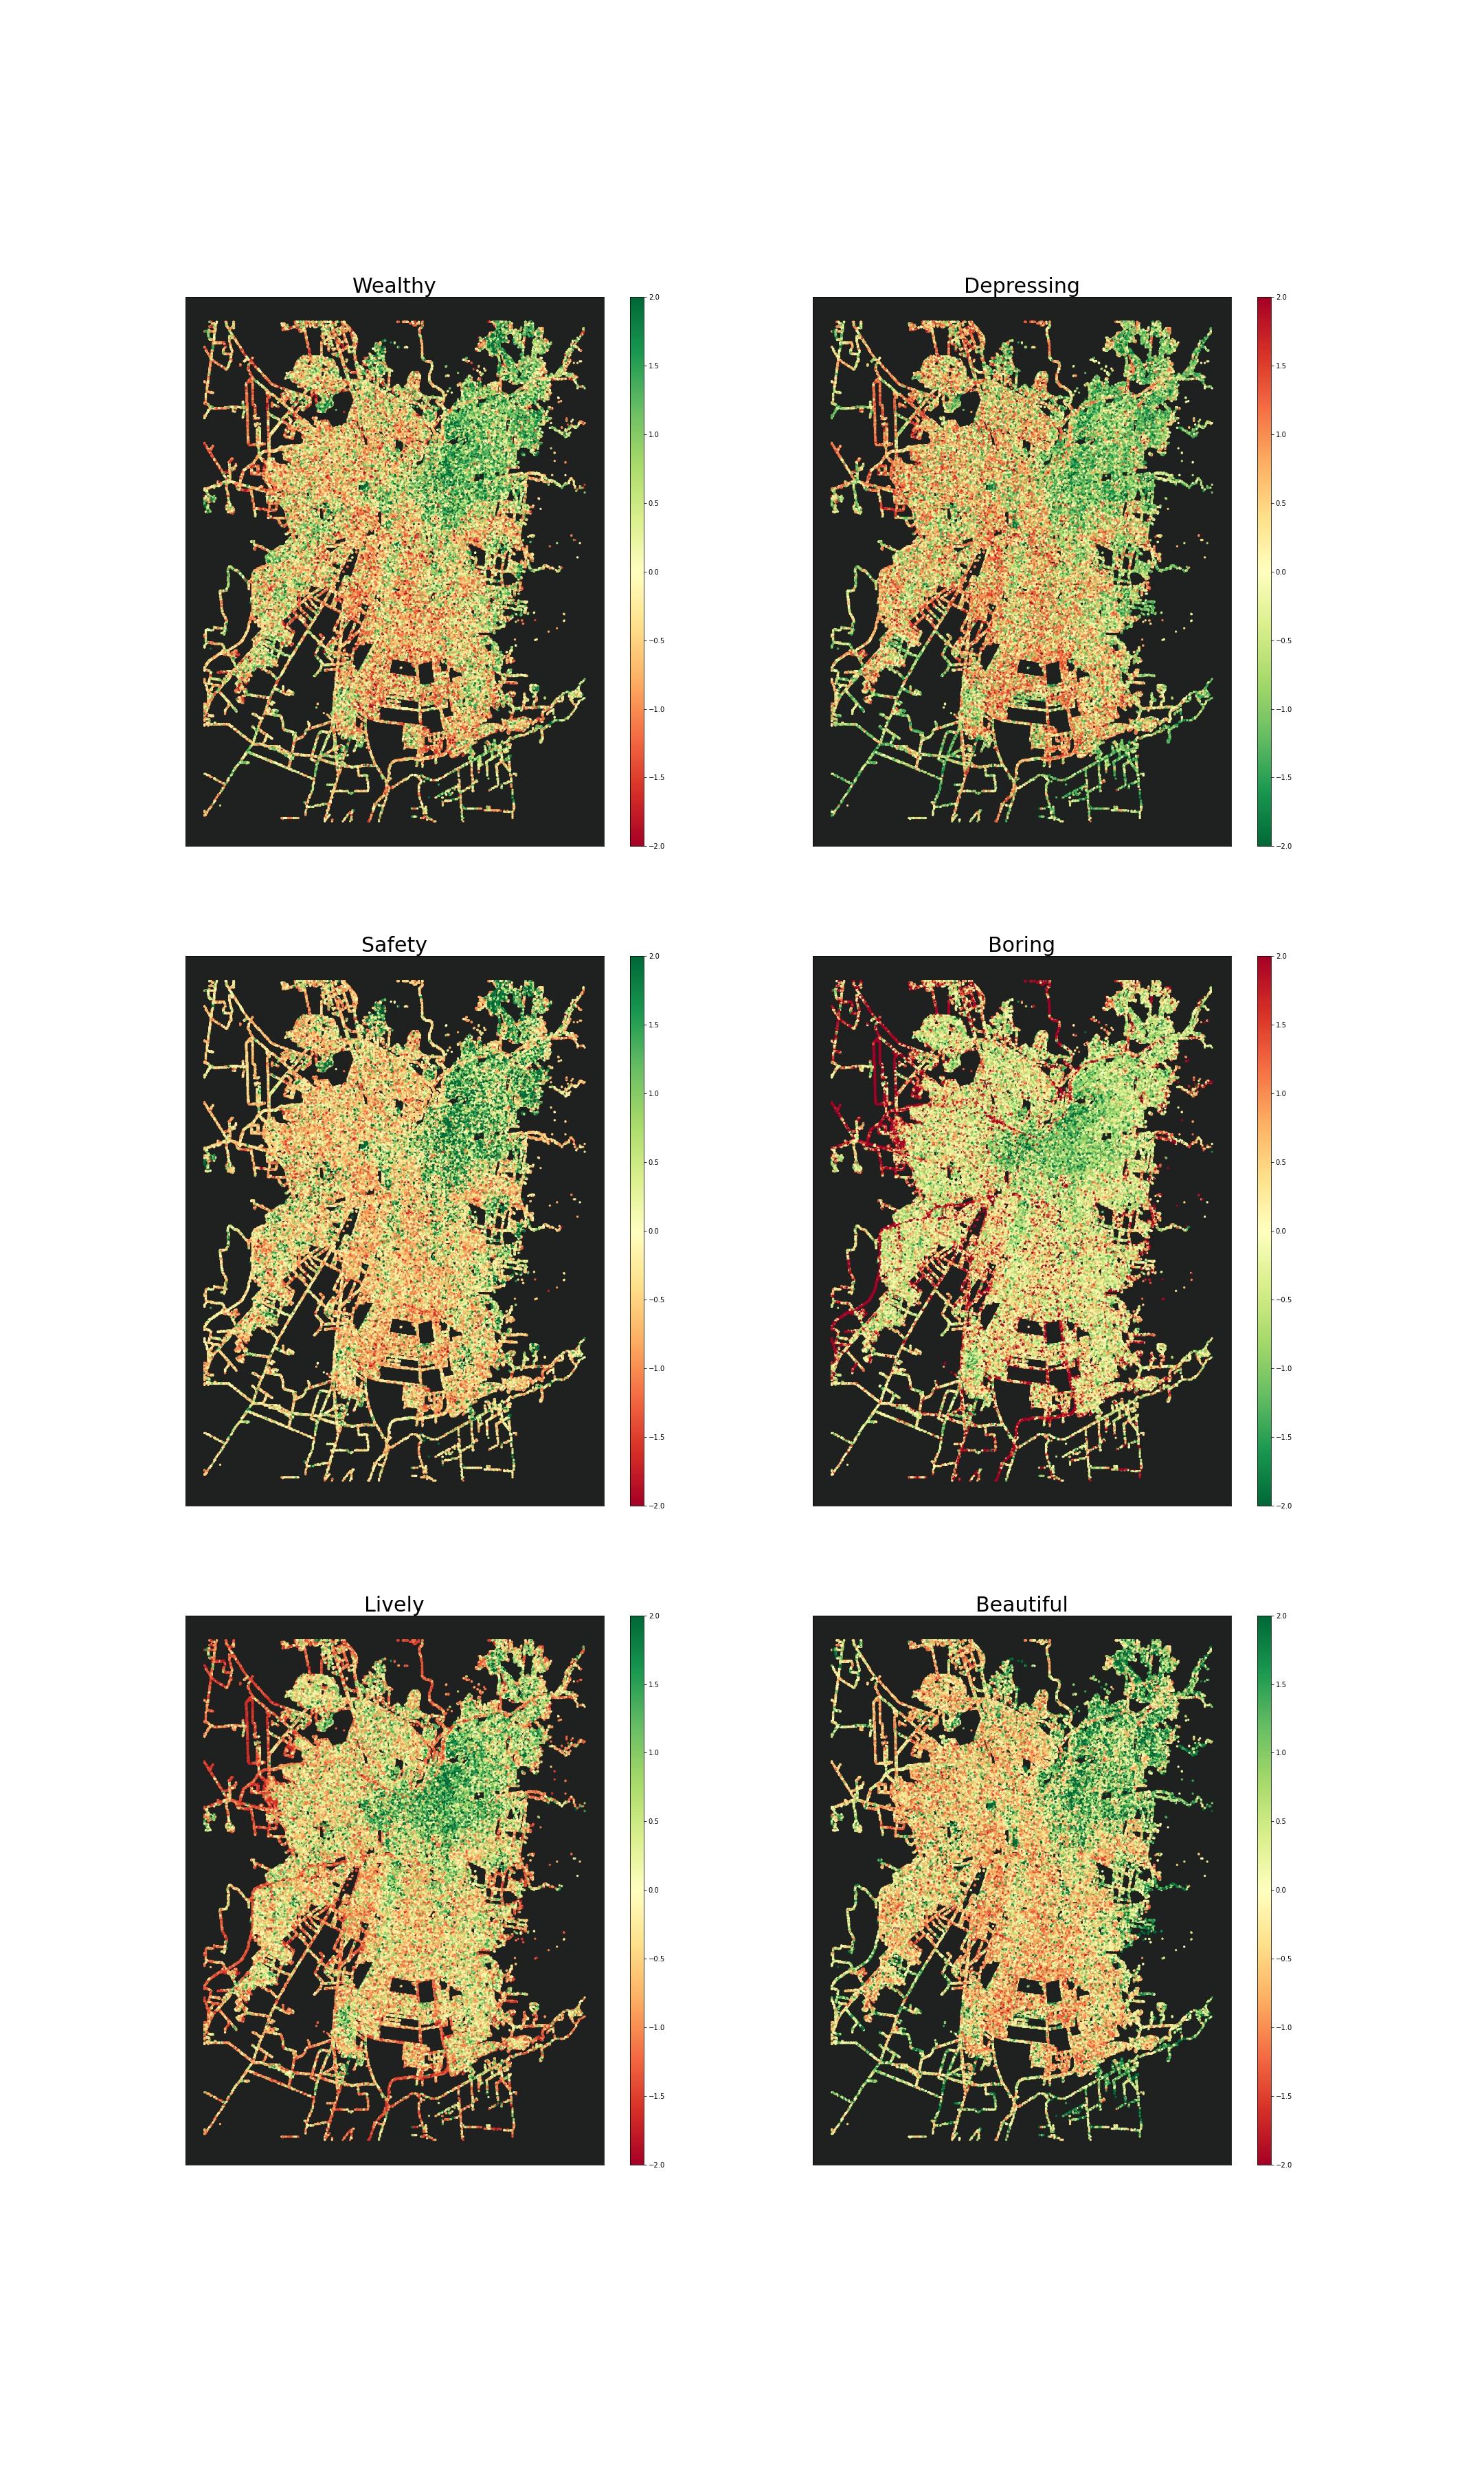
\includegraphics[width=0.75\textwidth]{./figures/colormaps.jpg}
	\caption[Urban Perception for Santiago de Chile]{
        Urban Perception for Santiago de Chile, each dot represents an image that
        was analyzed with our model.
    }
	\label{fig:colormaps}
	\end{center}
\end{figure}


\begin{figure}[ht]
	\begin{center}
	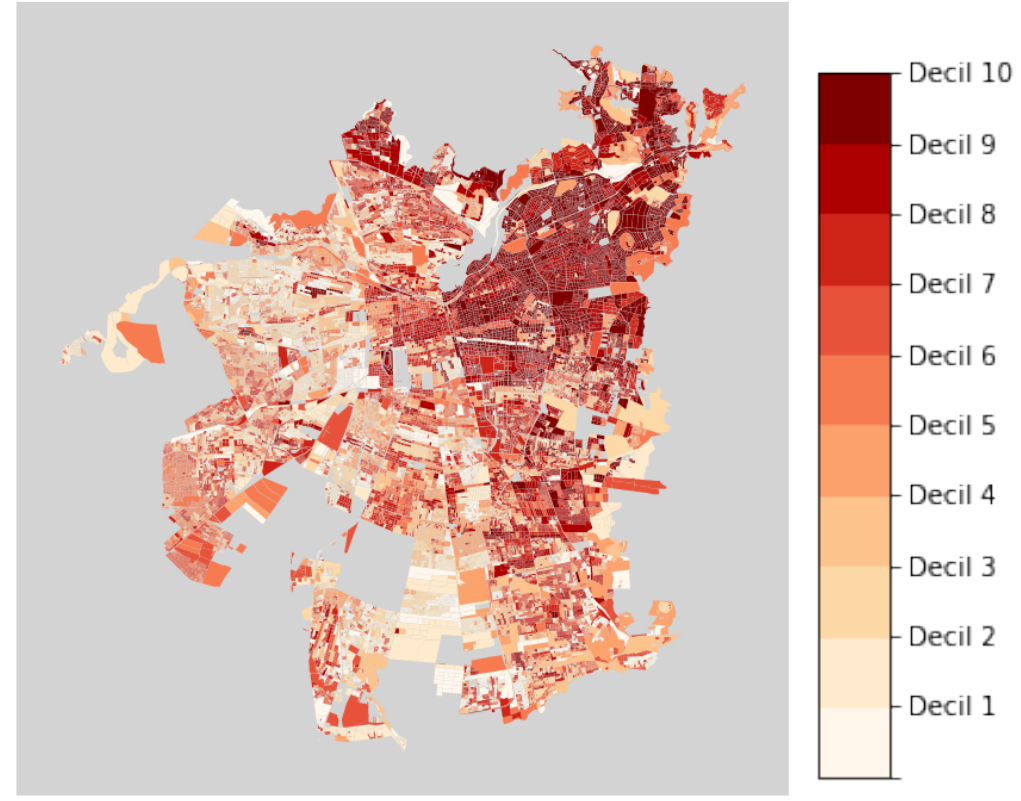
\includegraphics[width=0.75\textwidth]{./figures/eod.png}
	\caption[Wealth distribution of Santiago de Chile]{
        Wealth distribution of Santiago de Chile by deciles. Darker means wealthier.
        Reproduced from \citeA{Ramirez2020}.
    }
	\label{fig:eod}
	\end{center}
\end{figure}

In order to have a quantitative measure of the ranking generated for Santiago we calculate the mean score over
the images of each commune in the city and compare the results with their respective
socioeconomic indicators. We find a strong correlation between our perceived wealthy score
and the poverty rate, and between our perceived depressiveness score and social vulnerability.
We show this results on figures \ref{fig:poverty} and \ref{fig:vulnerability}.

\begin{figure}[ht]
	\begin{center}
	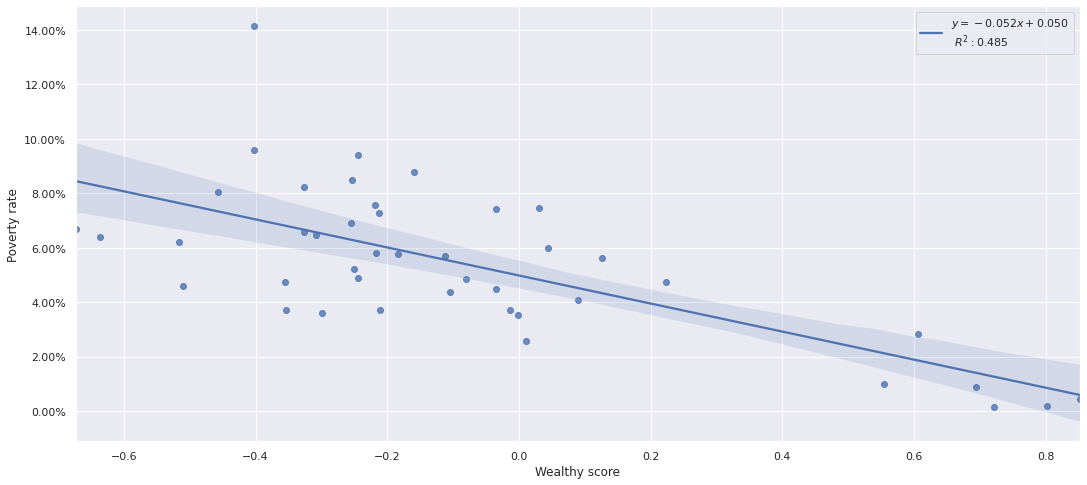
\includegraphics[width=0.75\textwidth]{./figures/poverty_rate.png}
	\caption[Poverty rate vs perceived wealthy score]{
		Poverty rate vs perceived wealthy score by commune in Santiago de Chile.
		Data taken from \citeA{casen}.
    }
	\label{fig:poverty}
	\end{center}
\end{figure}

\begin{figure}[ht]
	\begin{center}
	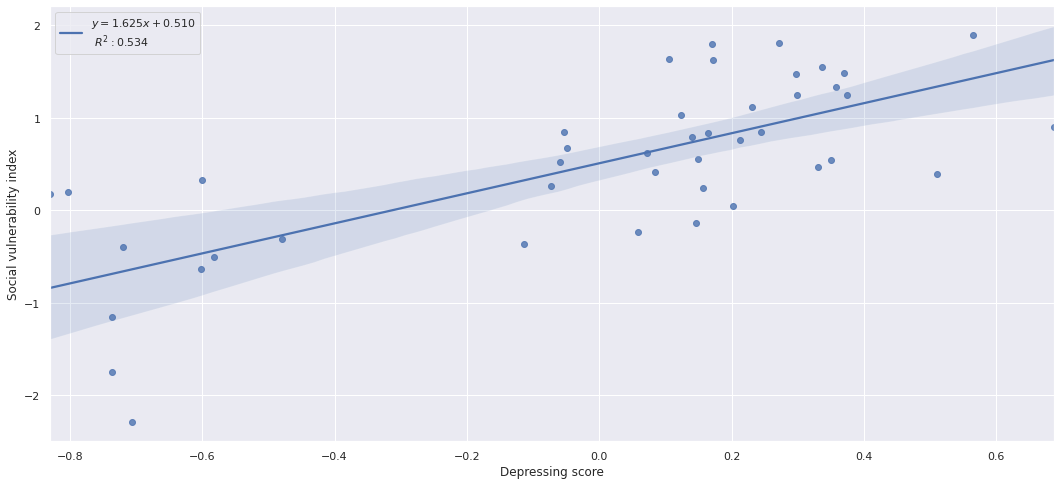
\includegraphics[width=0.75\textwidth]{./figures/vulnerability_index.png}
	\caption[Vulnerability index vs perceived depressiveness score]{
		Vulnerability index vs perceived depressiveness score by commune in Santiago de Chile.
		Data taken from \citeA{amuch}.
    }
	\label{fig:vulnerability}
	\end{center}
\end{figure}